\chapter{Introduction}

\anno{ca. 5 Seiten (2)}

Every operator of applications on the Internet, from small blogs to large business applications, is also exposed to the risk that potential attackers will try to disrupt or manipulate operations. The protection of applications in the area of IT security is therefore a necessity, but is usually not part of the core business of these users. For the most part, they rely on the fact that the application in operation is protected against all possible attack vectors. When analysing requirements, business users focus on the implementation of their business processes. In many cases, the precise location of an input field or the form and colour of a confirmation button are defined meticulously. But when it comes to security, the motto is often as simple as \glqq\emph{The application must be secure}\grqq \\

Ultimately, there is no need to reinvent the wheel and software manufacturers are happy when simple, reusable solutions can be used for common problems.

Every year the OWASP Top Ten~\cite{owasp10} publishes a list of the most commonly exploited and known web application vulnerabilities. In most cases, an application is secured against such risks on an individual basis.
And often each individual risk is addressed separately.\\


\begin{figure}[h]
  \begin{center}
    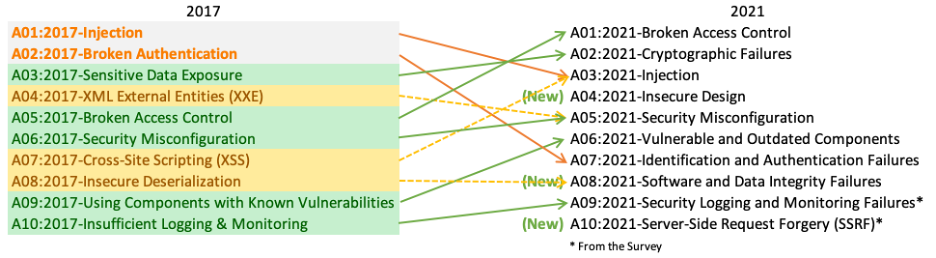
\includegraphics[width=15cm]{mapping}
    \caption{OWASP Top10 2017/2021~\cite{owasp10}}
    \label{fig.topten}
  \end{center}
\end{figure}

So-called \emph{Web application firewalls} (WAF) are a \emph{simple} and \emph{reusable} solution in the area of IT security for web-based applications. In the simplest case, these systems sit between the end user and the application that needs to be protected, listening to the data traffic and filtering out any harmful communication. The more a WAF knows about the applications to be protected, the easier it is for it to differentiate between \emph{harmful} and \emph{non-harmful} traffic. However, the configuration is often extensive and complex. The aim of this paper is to show how the configuration can be simplified in a practical way. Several systems or protecting applications are connected by a central component and can thus learn from each other. Web application firewalls (WAF) offer a relatively simple way to eliminate the majority of risks in general. However, the configuration of a web application firewall should be adapted to the application to be protected. \\

\anno{ggf. noch näher auf Angriffszenarien eingehen?}

% das grosse Problem
%% Was ist der Markt
%%% zahlreiche Anbieter teils spezialisiert auf bestimmte Bereiche; zahlreiche Arten von WAF
%% Wem hilft es?
%% Warum jetzt?
%% Ist das Problem lösbarer geworden?

\section{Aim of this work}
\label{sec:einleitungziel}
% Ziel der Arbeit
%% Was ist Ihr relevantes Teilproblem? Was ist die zentrale Frage?
%% Ihr Ziel in zwei Absätzen.
%%% Warum genau dieses Problem?
%%% Ist Ihr Beitrag völlig neu, oder nur ein Baustein?
%%% Ist Ihr Proble schwer zu lösen oder straight forward?
%%% Eher Forschung oder Anwendung?
%%% Was machen Sie nicht? Und warum haben Sie sich entschieden das nicht zu machen.
%% Wenn Sie ein System bauen...
%%% Welche Anfragen/Aufgaben wollen Sie beantworten/lösen können?
%%% Welche Kernfunktionalität soll Ihr System haben?
%%% Was ist ein typischer (Bedienungs-)Prozess für Ihr System

The aim of this thesis is to provide a way of integrating this protective measure more easily. As an example, a prototype including a test environment based on legacy WAF software is developed and then tested with the help of selected applications and attack patterns.  It is shown how the software is updated and how several instances of this software can be linked. The integration of a function for independent classification should relieve the user of complicated, individual configurations and provide a gain in security for web applications. A major problem in achieving this goal, however, is the limited availability of (public) data, as this has so far only been geared towards individual special cases or no longer corresponds to the current state of the art. The key questions are therefore:


\begin{itemize}
\item How do you get the most up-to-date and the most new data as possible?
\item What measures can be taken to significantly improve the quality of the data?
\item Can the data be exchanged as quickly as possible?
\end{itemize}


By answering these questions, it should be possible to increase the security of an application even without detailed knowledge of its internal structure.\\

\textcolor{bhtGray}{\ding{110} Thesis:} An application can also be secured with sufficient available data from similar applications!\\

This work is partly based on preliminary work in the field of application security, which is presented in more detail in the chapter \glqq\emph{Basics}\grqq{}.

% Methodik (1 Seite)
%% Wie wollen Sie das Problem lösen?
%% Welche Grundlagen müssen Sie beachten?
%% Wie ist Ihre Vorgehensweise?

% Gliederung und Aufbau (ca. 0,5 Seiten)
%% Wann lesen wir was und warum?
\section{Thesis structure}

% erster Teile Grundbegriffe, verwandte Vorarbeiten und

Dieses \textbf{erste Kapitel} der Arbeit lieferte bereits einen kurzen Einblick in die Thematik. Das folgende \textbf{zweite Kapitel} erläutert noch wichtige Grundbegriffe aus den Bereichen der IT-Sicherheit die zum Verständnis der Thematik beitragen, gefolgt von einer kurzen zeitlichen Einordnung zur Entwicklung der Web Application Firewalls in den letzten Jahren. Dabei wird insbesondere auf die Entwicklung von einfachen regelbasierten hin zu intelligenten Systemen eingegangen. Das folgende, dritte Kapitel enthält die Kernelemente der Arbeit und schlägt mögliche Verbesserungen und Erweiterungen vor. Der derzeitige Stand wird genauer betrachtet und mögliche Probleme mit Vorschlägen zu deren Lösung aufgezeigt. \textbf{Kapitel 4} gibt einen kurzen Einblick über stattgefundene Arbeiten zur technischen Umsetzung der Vorschläge aus dem vorhergehenden Kapitel anhand einer real existierenden Software. Im anschließenden Kapitel wird die Anwendung der entstandenen Lösung im Testumfeld erprobt und ausgewertet. Die Arbeit schließt mit einem kurzen Ausblick ab.

\section{Abgrenzung}

Diese Arbeit beschäftigt sich mit der Erweiterung eines bereits bestehenden Produktes und soll anhand praktischer Beispiele Möglichkeiten zur Verbesserung aufzeigen. Die in der Arbeit erwähnten Konzepte und Strategien lassen sich sicherlich auch auf andere Produkte übertragen, dieses soll jedoch nicht Inhalt in dieser Arbeit sein. Ein vollständiges Softwareprodukt mit der Möglichkeit zur Auslieferung an Endkunden ist ebenso wenig Teil dieser Arbeit. Eine Entwicklung bis zu einem (zufriedenstellenden) Auslieferungszustand würde den möglichen Zeitrahmen überschreiten. Stattdessen soll diese Arbeit Ideen und Anregungen für eine zukünftige Weiterentwicklung des Produktes liefern.
